% Options for packages loaded elsewhere
\PassOptionsToPackage{unicode}{hyperref}
\PassOptionsToPackage{hyphens}{url}
%
\documentclass[
]{article}
\title{Hands on Programming}
\author{Keefe Reuther}
\date{10/26/2021}

\usepackage{amsmath,amssymb}
\usepackage{lmodern}
\usepackage{iftex}
\ifPDFTeX
  \usepackage[T1]{fontenc}
  \usepackage[utf8]{inputenc}
  \usepackage{textcomp} % provide euro and other symbols
\else % if luatex or xetex
  \usepackage{unicode-math}
  \defaultfontfeatures{Scale=MatchLowercase}
  \defaultfontfeatures[\rmfamily]{Ligatures=TeX,Scale=1}
\fi
% Use upquote if available, for straight quotes in verbatim environments
\IfFileExists{upquote.sty}{\usepackage{upquote}}{}
\IfFileExists{microtype.sty}{% use microtype if available
  \usepackage[]{microtype}
  \UseMicrotypeSet[protrusion]{basicmath} % disable protrusion for tt fonts
}{}
\makeatletter
\@ifundefined{KOMAClassName}{% if non-KOMA class
  \IfFileExists{parskip.sty}{%
    \usepackage{parskip}
  }{% else
    \setlength{\parindent}{0pt}
    \setlength{\parskip}{6pt plus 2pt minus 1pt}}
}{% if KOMA class
  \KOMAoptions{parskip=half}}
\makeatother
\usepackage{xcolor}
\IfFileExists{xurl.sty}{\usepackage{xurl}}{} % add URL line breaks if available
\IfFileExists{bookmark.sty}{\usepackage{bookmark}}{\usepackage{hyperref}}
\hypersetup{
  pdftitle={Hands on Programming},
  pdfauthor={Keefe Reuther},
  hidelinks,
  pdfcreator={LaTeX via pandoc}}
\urlstyle{same} % disable monospaced font for URLs
\usepackage[margin=1in]{geometry}
\usepackage{color}
\usepackage{fancyvrb}
\newcommand{\VerbBar}{|}
\newcommand{\VERB}{\Verb[commandchars=\\\{\}]}
\DefineVerbatimEnvironment{Highlighting}{Verbatim}{commandchars=\\\{\}}
% Add ',fontsize=\small' for more characters per line
\usepackage{framed}
\definecolor{shadecolor}{RGB}{248,248,248}
\newenvironment{Shaded}{\begin{snugshade}}{\end{snugshade}}
\newcommand{\AlertTok}[1]{\textcolor[rgb]{0.94,0.16,0.16}{#1}}
\newcommand{\AnnotationTok}[1]{\textcolor[rgb]{0.56,0.35,0.01}{\textbf{\textit{#1}}}}
\newcommand{\AttributeTok}[1]{\textcolor[rgb]{0.77,0.63,0.00}{#1}}
\newcommand{\BaseNTok}[1]{\textcolor[rgb]{0.00,0.00,0.81}{#1}}
\newcommand{\BuiltInTok}[1]{#1}
\newcommand{\CharTok}[1]{\textcolor[rgb]{0.31,0.60,0.02}{#1}}
\newcommand{\CommentTok}[1]{\textcolor[rgb]{0.56,0.35,0.01}{\textit{#1}}}
\newcommand{\CommentVarTok}[1]{\textcolor[rgb]{0.56,0.35,0.01}{\textbf{\textit{#1}}}}
\newcommand{\ConstantTok}[1]{\textcolor[rgb]{0.00,0.00,0.00}{#1}}
\newcommand{\ControlFlowTok}[1]{\textcolor[rgb]{0.13,0.29,0.53}{\textbf{#1}}}
\newcommand{\DataTypeTok}[1]{\textcolor[rgb]{0.13,0.29,0.53}{#1}}
\newcommand{\DecValTok}[1]{\textcolor[rgb]{0.00,0.00,0.81}{#1}}
\newcommand{\DocumentationTok}[1]{\textcolor[rgb]{0.56,0.35,0.01}{\textbf{\textit{#1}}}}
\newcommand{\ErrorTok}[1]{\textcolor[rgb]{0.64,0.00,0.00}{\textbf{#1}}}
\newcommand{\ExtensionTok}[1]{#1}
\newcommand{\FloatTok}[1]{\textcolor[rgb]{0.00,0.00,0.81}{#1}}
\newcommand{\FunctionTok}[1]{\textcolor[rgb]{0.00,0.00,0.00}{#1}}
\newcommand{\ImportTok}[1]{#1}
\newcommand{\InformationTok}[1]{\textcolor[rgb]{0.56,0.35,0.01}{\textbf{\textit{#1}}}}
\newcommand{\KeywordTok}[1]{\textcolor[rgb]{0.13,0.29,0.53}{\textbf{#1}}}
\newcommand{\NormalTok}[1]{#1}
\newcommand{\OperatorTok}[1]{\textcolor[rgb]{0.81,0.36,0.00}{\textbf{#1}}}
\newcommand{\OtherTok}[1]{\textcolor[rgb]{0.56,0.35,0.01}{#1}}
\newcommand{\PreprocessorTok}[1]{\textcolor[rgb]{0.56,0.35,0.01}{\textit{#1}}}
\newcommand{\RegionMarkerTok}[1]{#1}
\newcommand{\SpecialCharTok}[1]{\textcolor[rgb]{0.00,0.00,0.00}{#1}}
\newcommand{\SpecialStringTok}[1]{\textcolor[rgb]{0.31,0.60,0.02}{#1}}
\newcommand{\StringTok}[1]{\textcolor[rgb]{0.31,0.60,0.02}{#1}}
\newcommand{\VariableTok}[1]{\textcolor[rgb]{0.00,0.00,0.00}{#1}}
\newcommand{\VerbatimStringTok}[1]{\textcolor[rgb]{0.31,0.60,0.02}{#1}}
\newcommand{\WarningTok}[1]{\textcolor[rgb]{0.56,0.35,0.01}{\textbf{\textit{#1}}}}
\usepackage{longtable,booktabs,array}
\usepackage{calc} % for calculating minipage widths
% Correct order of tables after \paragraph or \subparagraph
\usepackage{etoolbox}
\makeatletter
\patchcmd\longtable{\par}{\if@noskipsec\mbox{}\fi\par}{}{}
\makeatother
% Allow footnotes in longtable head/foot
\IfFileExists{footnotehyper.sty}{\usepackage{footnotehyper}}{\usepackage{footnote}}
\makesavenoteenv{longtable}
\usepackage{graphicx}
\makeatletter
\def\maxwidth{\ifdim\Gin@nat@width>\linewidth\linewidth\else\Gin@nat@width\fi}
\def\maxheight{\ifdim\Gin@nat@height>\textheight\textheight\else\Gin@nat@height\fi}
\makeatother
% Scale images if necessary, so that they will not overflow the page
% margins by default, and it is still possible to overwrite the defaults
% using explicit options in \includegraphics[width, height, ...]{}
\setkeys{Gin}{width=\maxwidth,height=\maxheight,keepaspectratio}
% Set default figure placement to htbp
\makeatletter
\def\fps@figure{htbp}
\makeatother
\setlength{\emergencystretch}{3em} % prevent overfull lines
\providecommand{\tightlist}{%
  \setlength{\itemsep}{0pt}\setlength{\parskip}{0pt}}
\setcounter{secnumdepth}{-\maxdimen} % remove section numbering
\ifLuaTeX
  \usepackage{selnolig}  % disable illegal ligatures
\fi

\begin{document}
\maketitle

\hypertarget{hands-on-programming}{%
\subsection{Hands On Programming}\label{hands-on-programming}}

\hypertarget{by-garrett-grolemund}{%
\subsubsection{by Garrett Grolemund}\label{by-garrett-grolemund}}

\url{https://rstudio-education.github.io/hopr/}

\hypertarget{introduction}{%
\subsubsection{Introduction}\label{introduction}}

Busses are very easy to use, you just need to know which bus to get on,
where to get on, and where to get off (and you need to pay your fare).
Cars, on the other hand, require much more work: you need to have some
type of map or directions (even if the map is in your head), you need to
put gas in every now and then, you need to know the rules of the road
(have some type of drivers license). The big advantage of the car is
that it can take you a bunch of places that the bus does not go and it
is quicker for some trips that would require transferring between
busses. Using this analogy, programs like SPSS are busses, easy to use
for the standard things, but very frustrating if you want to do
something that is not already preprogrammed. R is a 4-wheel drive SUV
(though environmentally friendly) with a bike on the back, a kayak on
top, good walking and running shoes in the passenger seat, and mountain
climbing and spelunking gear in the back. R can take you anywhere you
want to go if you take time to learn how to use the equipment, but that
is going to take longer than learning where the bus stops are in SPSS. -
Greg Snow

\hypertarget{project-1}{%
\subsubsection{Project 1}\label{project-1}}

You will learn to:

\begin{itemize}
\tightlist
\item
  Run R commands
\item
  Create R objects
\item
  Write your own R functions and scripts
\item
  Load and use R packages
\item
  Generate random samples
\item
  Create quick plots
\item
  Get help when you need it
\end{itemize}

\begin{Shaded}
\begin{Highlighting}[]
\DecValTok{1}\SpecialCharTok{+}\DecValTok{1}
\end{Highlighting}
\end{Shaded}

\begin{verbatim}
## [1] 2
\end{verbatim}

\begin{Shaded}
\begin{Highlighting}[]
\DecValTok{100}\SpecialCharTok{:}\DecValTok{130}
\end{Highlighting}
\end{Shaded}

\begin{verbatim}
##  [1] 100 101 102 103 104 105 106 107 108 109 110 111 112 113 114 115 116 117 118
## [20] 119 120 121 122 123 124 125 126 127 128 129 130
\end{verbatim}

\begin{Shaded}
\begin{Highlighting}[]
\DecValTok{5} \SpecialCharTok{{-}} 
  \SpecialCharTok{+}\DecValTok{1}
\end{Highlighting}
\end{Shaded}

\begin{verbatim}
## [1] 4
\end{verbatim}

\begin{Shaded}
\begin{Highlighting}[]
\DecValTok{237}\SpecialCharTok{+}\DecValTok{2}
\end{Highlighting}
\end{Shaded}

\begin{verbatim}
## [1] 239
\end{verbatim}

\begin{Shaded}
\begin{Highlighting}[]
\DecValTok{239}\SpecialCharTok{*}\DecValTok{3}
\end{Highlighting}
\end{Shaded}

\begin{verbatim}
## [1] 717
\end{verbatim}

\begin{Shaded}
\begin{Highlighting}[]
\DecValTok{717{-}6}
\end{Highlighting}
\end{Shaded}

\begin{verbatim}
## [1] 711
\end{verbatim}

\begin{Shaded}
\begin{Highlighting}[]
\DecValTok{711}\SpecialCharTok{/}\DecValTok{3}
\end{Highlighting}
\end{Shaded}

\begin{verbatim}
## [1] 237
\end{verbatim}

\begin{Shaded}
\begin{Highlighting}[]
\DecValTok{1}\SpecialCharTok{:}\DecValTok{6}
\end{Highlighting}
\end{Shaded}

\begin{verbatim}
## [1] 1 2 3 4 5 6
\end{verbatim}

\begin{Shaded}
\begin{Highlighting}[]
\NormalTok{a }\OtherTok{\textless{}{-}} \DecValTok{1}
\NormalTok{a}
\end{Highlighting}
\end{Shaded}

\begin{verbatim}
## [1] 1
\end{verbatim}

\begin{Shaded}
\begin{Highlighting}[]
\NormalTok{a}\SpecialCharTok{*}\DecValTok{3}
\end{Highlighting}
\end{Shaded}

\begin{verbatim}
## [1] 3
\end{verbatim}

\begin{Shaded}
\begin{Highlighting}[]
\NormalTok{a}\SpecialCharTok{\^{}}\DecValTok{0}
\end{Highlighting}
\end{Shaded}

\begin{verbatim}
## [1] 1
\end{verbatim}

\begin{Shaded}
\begin{Highlighting}[]
\FunctionTok{round}\NormalTok{(}\FloatTok{3.14}\NormalTok{, }\AttributeTok{digits=}\DecValTok{1}\NormalTok{)}
\end{Highlighting}
\end{Shaded}

\begin{verbatim}
## [1] 3.1
\end{verbatim}

\begin{Shaded}
\begin{Highlighting}[]
\FunctionTok{factorial}\NormalTok{(}\DecValTok{7}\NormalTok{)}
\end{Highlighting}
\end{Shaded}

\begin{verbatim}
## [1] 5040
\end{verbatim}

\hypertarget{including-plots}{%
\subsubsection{Including Plots}\label{including-plots}}

\begin{Shaded}
\begin{Highlighting}[]
\NormalTok{die }\OtherTok{\textless{}{-}} \DecValTok{1}\SpecialCharTok{:}\DecValTok{6}
\NormalTok{die}
\end{Highlighting}
\end{Shaded}

\begin{verbatim}
## [1] 1 2 3 4 5 6
\end{verbatim}

\begin{Shaded}
\begin{Highlighting}[]
\FunctionTok{ls}\NormalTok{()}
\end{Highlighting}
\end{Shaded}

\begin{verbatim}
## [1] "a"   "die"
\end{verbatim}

\begin{Shaded}
\begin{Highlighting}[]
\NormalTok{die }\SpecialCharTok{{-}} \DecValTok{1}
\end{Highlighting}
\end{Shaded}

\begin{verbatim}
## [1] 0 1 2 3 4 5
\end{verbatim}

\begin{Shaded}
\begin{Highlighting}[]
\NormalTok{die }\SpecialCharTok{/} \DecValTok{2}
\end{Highlighting}
\end{Shaded}

\begin{verbatim}
## [1] 0.5 1.0 1.5 2.0 2.5 3.0
\end{verbatim}

\begin{Shaded}
\begin{Highlighting}[]
\NormalTok{die }\SpecialCharTok{*}\NormalTok{ die}
\end{Highlighting}
\end{Shaded}

\begin{verbatim}
## [1]  1  4  9 16 25 36
\end{verbatim}

\begin{Shaded}
\begin{Highlighting}[]
\NormalTok{die }\SpecialCharTok{\%*\%}\NormalTok{ die}
\end{Highlighting}
\end{Shaded}

\begin{verbatim}
##      [,1]
## [1,]   91
\end{verbatim}

\begin{Shaded}
\begin{Highlighting}[]
\NormalTok{die }\SpecialCharTok{\%o\%}\NormalTok{ die}
\end{Highlighting}
\end{Shaded}

\begin{verbatim}
##      [,1] [,2] [,3] [,4] [,5] [,6]
## [1,]    1    2    3    4    5    6
## [2,]    2    4    6    8   10   12
## [3,]    3    6    9   12   15   18
## [4,]    4    8   12   16   20   24
## [5,]    5   10   15   20   25   30
## [6,]    6   12   18   24   30   36
\end{verbatim}

\begin{Shaded}
\begin{Highlighting}[]
\FunctionTok{mean}\NormalTok{(die)}
\end{Highlighting}
\end{Shaded}

\begin{verbatim}
## [1] 3.5
\end{verbatim}

\begin{Shaded}
\begin{Highlighting}[]
\FunctionTok{sample}\NormalTok{(die, }\DecValTok{10}\NormalTok{, }\AttributeTok{replace =} \ConstantTok{TRUE}\NormalTok{)}
\end{Highlighting}
\end{Shaded}

\begin{verbatim}
##  [1] 5 1 2 5 4 1 1 3 3 6
\end{verbatim}

\begin{Shaded}
\begin{Highlighting}[]
\FunctionTok{args}\NormalTok{(sample)}
\end{Highlighting}
\end{Shaded}

\begin{verbatim}
## function (x, size, replace = FALSE, prob = NULL) 
## NULL
\end{verbatim}

\begin{Shaded}
\begin{Highlighting}[]
\NormalTok{dice }\OtherTok{\textless{}{-}}  \FunctionTok{sample}\NormalTok{(die, }\DecValTok{10}\NormalTok{, }\AttributeTok{replace =} \ConstantTok{TRUE}\NormalTok{)}
\NormalTok{dice}
\end{Highlighting}
\end{Shaded}

\begin{verbatim}
##  [1] 1 5 4 1 4 5 5 5 6 1
\end{verbatim}

\begin{Shaded}
\begin{Highlighting}[]
\FunctionTok{sum}\NormalTok{(dice)}
\end{Highlighting}
\end{Shaded}

\begin{verbatim}
## [1] 37
\end{verbatim}

\begin{figure}
\centering
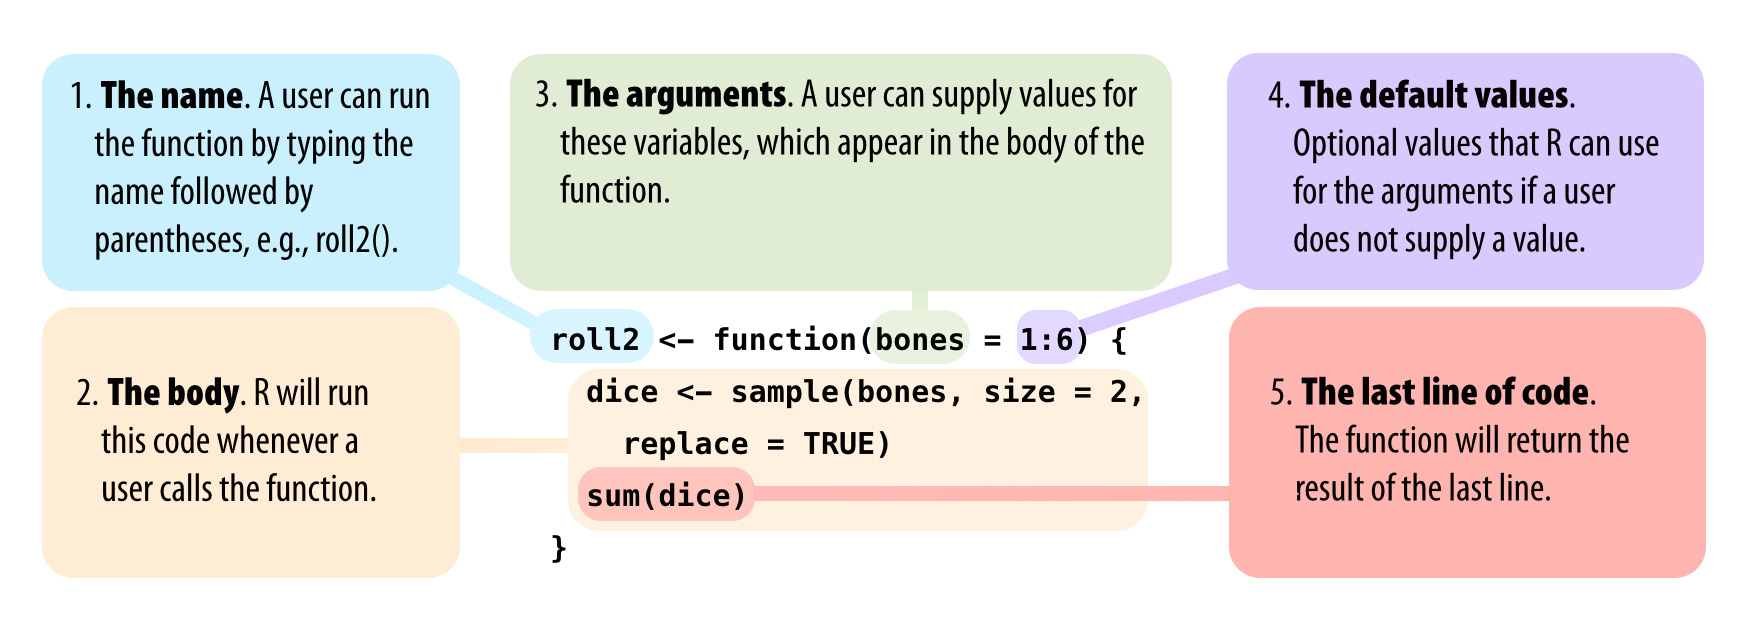
\includegraphics{~/BILD 5 sandbox/Hands_on_programming/hopr_0106.png}
\caption{parts of a function}
\end{figure}

\hypertarget{making-your-own-functions}{%
\subsubsection{Making your own
functions}\label{making-your-own-functions}}

\begin{Shaded}
\begin{Highlighting}[]
\NormalTok{my\_function }\OtherTok{\textless{}{-}} \ControlFlowTok{function}\NormalTok{() \{}
\NormalTok{  die }\OtherTok{\textless{}{-}} \DecValTok{1}\SpecialCharTok{:}\DecValTok{6}
\NormalTok{  dice }\OtherTok{\textless{}{-}} \FunctionTok{sample}\NormalTok{(die, }\AttributeTok{size =} \DecValTok{2}\NormalTok{, }\AttributeTok{replace =} \ConstantTok{TRUE}\NormalTok{)}
  \FunctionTok{sum}\NormalTok{(dice)}
\NormalTok{\}}
\FunctionTok{my\_function}\NormalTok{()}
\end{Highlighting}
\end{Shaded}

\begin{verbatim}
## [1] 9
\end{verbatim}

\begin{Shaded}
\begin{Highlighting}[]
\FunctionTok{my\_function}\NormalTok{()}
\end{Highlighting}
\end{Shaded}

\begin{verbatim}
## [1] 7
\end{verbatim}

\begin{Shaded}
\begin{Highlighting}[]
\NormalTok{roll }\OtherTok{\textless{}{-}} \FunctionTok{my\_function}\NormalTok{()}
\NormalTok{roll}
\end{Highlighting}
\end{Shaded}

\begin{verbatim}
## [1] 5
\end{verbatim}

\begin{Shaded}
\begin{Highlighting}[]
\NormalTok{roll}
\end{Highlighting}
\end{Shaded}

\begin{verbatim}
## [1] 5
\end{verbatim}

\begin{Shaded}
\begin{Highlighting}[]
\NormalTok{roll}
\end{Highlighting}
\end{Shaded}

\begin{verbatim}
## [1] 5
\end{verbatim}

\begin{Shaded}
\begin{Highlighting}[]
\FunctionTok{my\_function}\NormalTok{()}
\end{Highlighting}
\end{Shaded}

\begin{verbatim}
## [1] 4
\end{verbatim}

\begin{Shaded}
\begin{Highlighting}[]
\NormalTok{roll2 }\OtherTok{\textless{}{-}} \ControlFlowTok{function}\NormalTok{(bones) \{}
\NormalTok{  dice }\OtherTok{\textless{}{-}} \FunctionTok{sample}\NormalTok{(bones, }\AttributeTok{size =} \DecValTok{2}\NormalTok{, }\AttributeTok{replace =} \ConstantTok{TRUE}\NormalTok{)}
  \FunctionTok{sum}\NormalTok{(dice)}
\NormalTok{\}}
\FunctionTok{roll2}\NormalTok{(}\AttributeTok{bones =} \DecValTok{1}\SpecialCharTok{:}\DecValTok{100}\NormalTok{)}
\end{Highlighting}
\end{Shaded}

\begin{verbatim}
## [1] 144
\end{verbatim}

\begin{Shaded}
\begin{Highlighting}[]
\NormalTok{roll2 }\OtherTok{\textless{}{-}} \ControlFlowTok{function}\NormalTok{(}\AttributeTok{bones =} \DecValTok{1}\SpecialCharTok{:}\DecValTok{6}\NormalTok{) \{}
\NormalTok{  dice }\OtherTok{\textless{}{-}} \FunctionTok{sample}\NormalTok{(bones, }\AttributeTok{size =} \DecValTok{2}\NormalTok{, }\AttributeTok{replace =} \ConstantTok{TRUE}\NormalTok{)}
  \FunctionTok{sum}\NormalTok{(dice)}
\NormalTok{\}}
\NormalTok{roll2}
\end{Highlighting}
\end{Shaded}

\begin{verbatim}
## function(bones = 1:6) {
##   dice <- sample(bones, size = 2, replace = TRUE)
##   sum(dice)
## }
\end{verbatim}

\begin{Shaded}
\begin{Highlighting}[]
\FunctionTok{roll2}\NormalTok{()}
\end{Highlighting}
\end{Shaded}

\begin{verbatim}
## [1] 4
\end{verbatim}

\hypertarget{making-plots-and-getting-packages}{%
\subsubsection{Making plots and getting
packages}\label{making-plots-and-getting-packages}}

\begin{Shaded}
\begin{Highlighting}[]
\FunctionTok{library}\NormalTok{(}\StringTok{"ggplot2"}\NormalTok{)}
\NormalTok{x }\OtherTok{\textless{}{-}} \FunctionTok{c}\NormalTok{(}\DecValTok{1}\NormalTok{, }\DecValTok{2}\NormalTok{, }\FloatTok{3.4}\NormalTok{, }\SpecialCharTok{{-}}\FloatTok{0.8}\NormalTok{, }\DecValTok{2}\NormalTok{, }\SpecialCharTok{{-}}\DecValTok{3}\NormalTok{, }\DecValTok{3}\NormalTok{, }\DecValTok{4}\NormalTok{, }\DecValTok{6}\NormalTok{, }\DecValTok{8}\NormalTok{)}
\NormalTok{y }\OtherTok{\textless{}{-}}\NormalTok{ x}\SpecialCharTok{\^{}}\DecValTok{2}
\FunctionTok{qplot}\NormalTok{(x, y)}
\end{Highlighting}
\end{Shaded}

\includegraphics{hands_on_files/figure-latex/unnamed-chunk-4-1.pdf}

\begin{Shaded}
\begin{Highlighting}[]
\NormalTok{x }\OtherTok{\textless{}{-}} \FunctionTok{c}\NormalTok{(}\DecValTok{1}\NormalTok{, }\DecValTok{2}\NormalTok{, }\DecValTok{2}\NormalTok{, }\DecValTok{2}\NormalTok{, }\DecValTok{3}\NormalTok{, }\DecValTok{3}\NormalTok{)}
\FunctionTok{qplot}\NormalTok{(x, }\AttributeTok{binwidth =} \DecValTok{1}\NormalTok{)}
\end{Highlighting}
\end{Shaded}

\includegraphics{hands_on_files/figure-latex/unnamed-chunk-4-2.pdf}

\begin{Shaded}
\begin{Highlighting}[]
\NormalTok{x2 }\OtherTok{\textless{}{-}} \FunctionTok{c}\NormalTok{(}\DecValTok{1}\NormalTok{,}\DecValTok{1}\NormalTok{,}\DecValTok{1}\NormalTok{,}\DecValTok{1}\NormalTok{,}\DecValTok{1}\NormalTok{,}\DecValTok{2}\NormalTok{,}\DecValTok{2}\NormalTok{,}\DecValTok{2}\NormalTok{,}\DecValTok{2}\NormalTok{,}\DecValTok{3}\NormalTok{,}\DecValTok{3}\NormalTok{,}\DecValTok{4}\NormalTok{)}
\FunctionTok{qplot}\NormalTok{(x2, }\AttributeTok{binwidth =} \DecValTok{1}\NormalTok{)}
\end{Highlighting}
\end{Shaded}

\includegraphics{hands_on_files/figure-latex/unnamed-chunk-4-3.pdf}

\begin{Shaded}
\begin{Highlighting}[]
\NormalTok{lots }\OtherTok{\textless{}{-}} \FunctionTok{replicate}\NormalTok{(}\DecValTok{1000}\NormalTok{,}\FunctionTok{my\_function}\NormalTok{() )}
\FunctionTok{qplot}\NormalTok{(lots, }\AttributeTok{binwidth =} \FloatTok{0.5}\NormalTok{)}
\end{Highlighting}
\end{Shaded}

\includegraphics{hands_on_files/figure-latex/unnamed-chunk-4-4.pdf}

\begin{Shaded}
\begin{Highlighting}[]
\NormalTok{?sample}
\NormalTok{lots }\OtherTok{\textless{}{-}} \FunctionTok{replicate}\NormalTok{(}\DecValTok{10000}\NormalTok{,}\FunctionTok{my\_function}\NormalTok{() )}
\FunctionTok{qplot}\NormalTok{(lots, }\AttributeTok{binwidth =} \FloatTok{0.5}\NormalTok{)}
\end{Highlighting}
\end{Shaded}

\includegraphics{hands_on_files/figure-latex/unnamed-chunk-4-5.pdf}

\#\#\#Make your own function

Create a function where the die roll is unevenly weighted to roll a six
50\% of the time.

\begin{Shaded}
\begin{Highlighting}[]
\NormalTok{my\_function}
\end{Highlighting}
\end{Shaded}

\begin{verbatim}
## function() {
##   die <- 1:6
##   dice <- sample(die, size = 2, replace = TRUE)
##   sum(dice)
## }
## <bytecode: 0x55e1236bdf18>
\end{verbatim}

\begin{Shaded}
\begin{Highlighting}[]
\NormalTok{unfair\_dice }\OtherTok{\textless{}{-}} \ControlFlowTok{function}\NormalTok{() \{}
\NormalTok{  die }\OtherTok{\textless{}{-}} \DecValTok{1}\SpecialCharTok{:}\DecValTok{6}
\NormalTok{  unfair }\OtherTok{\textless{}{-}} \FunctionTok{sample}\NormalTok{(die, }\AttributeTok{size =} \DecValTok{1}\NormalTok{, }\AttributeTok{replace =} \ConstantTok{TRUE}\NormalTok{, }\AttributeTok{prob =} \FunctionTok{c}\NormalTok{(}\DecValTok{1}\NormalTok{,}\DecValTok{1}\NormalTok{,}\DecValTok{1}\NormalTok{,}\DecValTok{1}\NormalTok{,}\DecValTok{1}\NormalTok{,}\DecValTok{5}\NormalTok{))}
\NormalTok{\}}
\NormalTok{unfairresult }\OtherTok{\textless{}{-}} \FunctionTok{replicate}\NormalTok{(}\DecValTok{10000}\NormalTok{, }\FunctionTok{unfair\_dice}\NormalTok{())}
\FunctionTok{qplot}\NormalTok{(unfairresult, }\AttributeTok{binwidth =} \FloatTok{0.5}\NormalTok{)}
\end{Highlighting}
\end{Shaded}

\includegraphics{hands_on_files/figure-latex/unnamed-chunk-5-1.pdf}

This is the end of part 1 of \emph{Hands on Programming}

\#\#Part 2 \emph{Hands on Programming}

Along the way, you will learn how to:

\begin{itemize}
\tightlist
\item
  Save new types of data, like character strings and logical values
\item
  Save a data set as a vector, matrix, array, list, or data frame
\item
  Load and save your own data sets with R
\item
  Extract individual values from a data set
\item
  Change individual values within a data set
\item
  Write logical tests
\item
  Use R's missing-value symbol, NA
\end{itemize}

\#\#\#Tasks

\begin{enumerate}
\def\labelenumi{\arabic{enumi}.}
\tightlist
\item
  build the deck
\item
  write functions to deal and shuffle deck
\item
  change point system for game
\item
  manage state of deck
\end{enumerate}

An atomic vector is a ``c(x,\ldots..)'' . There are six basic types:

\begin{enumerate}
\def\labelenumi{\arabic{enumi}.}
\tightlist
\item
  doubles or numeric = regular numbers
\item
  integers = ``L'' following number
\item
  characters = input surrounded by ``\,'' = the individual elements are
  called strings
\item
  logicals = TRUE and FALSE and must be in CAPS
\item
  complex = complex numbers with i ``imaginary''
\item
  raw = straight up binary
\end{enumerate}

The most common attributes ``metadata'' to give a vector are:

\begin{itemize}
\tightlist
\item
  names = names(object) \textless- c(name1, name2,\ldots)
\item
  dimensions = dim(object) \textless- c(row\#, column\#)

  \begin{itemize}
  \tightlist
  \item
    m \textless- matrix(die, nrow = 2) fill with vector by column. Add
    ``byrow = TRUE'' if you want to add by row.
  \end{itemize}
\item
  class = ``class()'' can assign a class and ``unclass()'' can remove it

  \begin{itemize}
  \tightlist
  \item
    factors is one of the most important classes and stores categorical
    information that can be sorted
  \end{itemize}
\end{itemize}

A single vector can only have \textbf{1 data type}

Many data sets contain multiple types of information. The inability of
vectors, matrices, and arrays to store multiple data types seems like a
major limitation. So why bother with them?

In some cases, using only a single type of data is a huge advantage.
Vectors, matrices, and arrays make it very easy to do math on large sets
of numbers because R knows that it can manipulate each value the same
way. Operations with vectors, matrices, and arrays also tend to be fast
because the objects are so simple to store in memory.

In other cases, allowing only a single type of data is not a
disadvantage. Vectors are the most common data structure in R because
they store variables very well. Each value in a variable measures the
same property, so there's no need to use different types of data.

\#\#\#\#Lists list creates a list the same way c creates a vector.

Making a matrix of cards with 3 names = face suit value

\begin{Shaded}
\begin{Highlighting}[]
\NormalTok{cface }\OtherTok{\textless{}{-}} \FunctionTok{c}\NormalTok{(}\StringTok{"deuce"}\NormalTok{, }\StringTok{"ace"}\NormalTok{, }\StringTok{"king"}\NormalTok{, }\StringTok{"queen"}\NormalTok{, }\StringTok{"jack"}\NormalTok{, }\StringTok{"ten"}\NormalTok{, }\StringTok{"nine"}\NormalTok{, }\StringTok{"eight"}\NormalTok{, }\StringTok{"seven"}\NormalTok{, }\StringTok{"six"}\NormalTok{, }\StringTok{"five"}\NormalTok{, }\StringTok{"four"}\NormalTok{, }\StringTok{"three"}\NormalTok{)}
\NormalTok{csuit }\OtherTok{\textless{}{-}} \FunctionTok{c}\NormalTok{(}\StringTok{"spades"}\NormalTok{, }\StringTok{"hearts"}\NormalTok{, }\StringTok{"clubs"}\NormalTok{, }\StringTok{"diamonds"}\NormalTok{)}
\NormalTok{cvalue }\OtherTok{\textless{}{-}} \FunctionTok{c}\NormalTok{(}\DecValTok{15}\SpecialCharTok{:}\DecValTok{3}\NormalTok{)}
\NormalTok{clist }\OtherTok{\textless{}{-}} \FunctionTok{list}\NormalTok{(cface, csuit, cvalue)}
\NormalTok{clist}
\end{Highlighting}
\end{Shaded}

\begin{verbatim}
## [[1]]
##  [1] "deuce" "ace"   "king"  "queen" "jack"  "ten"   "nine"  "eight" "seven"
## [10] "six"   "five"  "four"  "three"
## 
## [[2]]
## [1] "spades"   "hearts"   "clubs"    "diamonds"
## 
## [[3]]
##  [1] 15 14 13 12 11 10  9  8  7  6  5  4  3
\end{verbatim}

\begin{Shaded}
\begin{Highlighting}[]
\FunctionTok{typeof}\NormalTok{(clist)}
\end{Highlighting}
\end{Shaded}

\begin{verbatim}
## [1] "list"
\end{verbatim}

\begin{Shaded}
\begin{Highlighting}[]
\FunctionTok{class}\NormalTok{(clist)}
\end{Highlighting}
\end{Shaded}

\begin{verbatim}
## [1] "list"
\end{verbatim}

\begin{Shaded}
\begin{Highlighting}[]
\FunctionTok{str}\NormalTok{(clist)}
\end{Highlighting}
\end{Shaded}

\begin{verbatim}
## List of 3
##  $ : chr [1:13] "deuce" "ace" "king" "queen" ...
##  $ : chr [1:4] "spades" "hearts" "clubs" "diamonds"
##  $ : int [1:13] 15 14 13 12 11 10 9 8 7 6 ...
\end{verbatim}

\#\#\#\#Data Frames

In this I am making a basic data frame but then making a full deck
using:

rep() to duplicate values in a vector (default is collated, otherwise
use ``each='' attribute) cbind() to add vectors or lists or dataframes
together

\begin{figure}
\centering
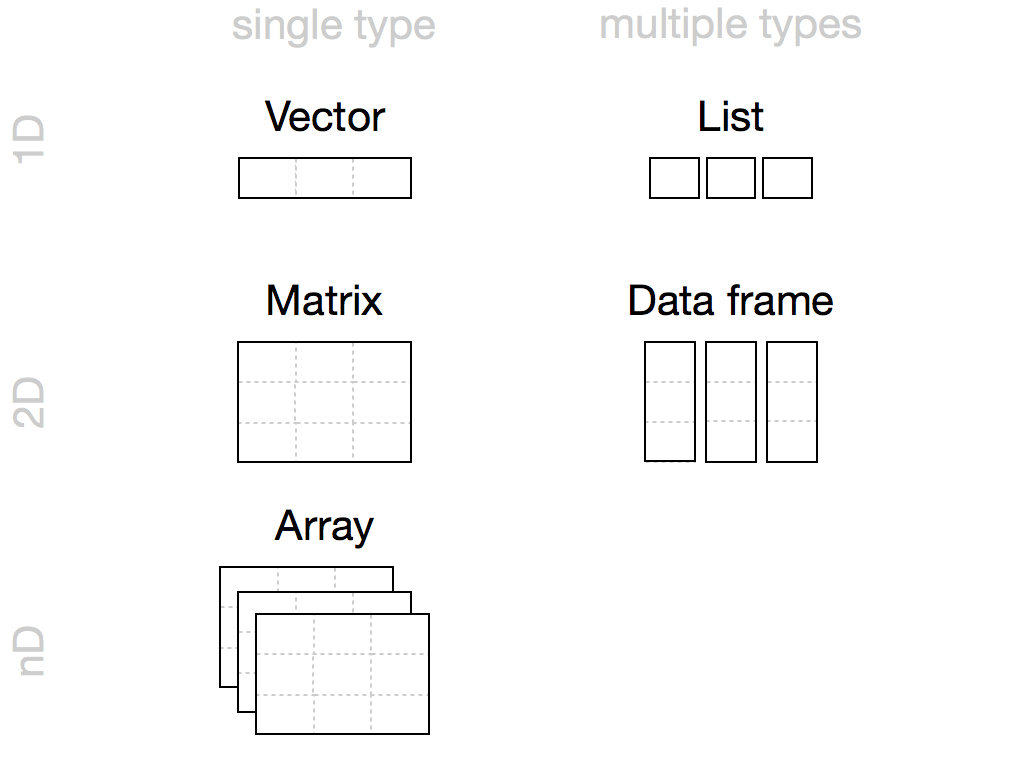
\includegraphics{~/BILD 5 sandbox/Hands_on_programming/hopr_0306.png}
\caption{types of data}
\end{figure}

\begin{Shaded}
\begin{Highlighting}[]
\NormalTok{df }\OtherTok{\textless{}{-}} \FunctionTok{data.frame}\NormalTok{(}\AttributeTok{face =} \FunctionTok{c}\NormalTok{(}\StringTok{"ace"}\NormalTok{, }\StringTok{"two"}\NormalTok{, }\StringTok{"six"}\NormalTok{),  }
  \AttributeTok{suit =} \FunctionTok{c}\NormalTok{(}\StringTok{"clubs"}\NormalTok{, }\StringTok{"clubs"}\NormalTok{, }\StringTok{"clubs"}\NormalTok{), }\AttributeTok{value =} \FunctionTok{c}\NormalTok{(}\DecValTok{1}\NormalTok{, }\DecValTok{2}\NormalTok{, }\DecValTok{3}\NormalTok{))}
\NormalTok{df}
\end{Highlighting}
\end{Shaded}

\begin{verbatim}
##   face  suit value
## 1  ace clubs     1
## 2  two clubs     2
## 3  six clubs     3
\end{verbatim}

\begin{Shaded}
\begin{Highlighting}[]
\FunctionTok{typeof}\NormalTok{(df)}
\end{Highlighting}
\end{Shaded}

\begin{verbatim}
## [1] "list"
\end{verbatim}

\begin{Shaded}
\begin{Highlighting}[]
\FunctionTok{class}\NormalTok{(df)}
\end{Highlighting}
\end{Shaded}

\begin{verbatim}
## [1] "data.frame"
\end{verbatim}

\begin{Shaded}
\begin{Highlighting}[]
\FunctionTok{str}\NormalTok{(df)}
\end{Highlighting}
\end{Shaded}

\begin{verbatim}
## 'data.frame':    3 obs. of  3 variables:
##  $ face : chr  "ace" "two" "six"
##  $ suit : chr  "clubs" "clubs" "clubs"
##  $ value: num  1 2 3
\end{verbatim}

\begin{Shaded}
\begin{Highlighting}[]
\NormalTok{cface }\OtherTok{\textless{}{-}} \FunctionTok{c}\NormalTok{(}\StringTok{"deuce"}\NormalTok{, }\StringTok{"ace"}\NormalTok{, }\StringTok{"king"}\NormalTok{, }\StringTok{"queen"}\NormalTok{, }\StringTok{"jack"}\NormalTok{, }\StringTok{"ten"}\NormalTok{, }\StringTok{"nine"}\NormalTok{, }\StringTok{"eight"}\NormalTok{, }\StringTok{"seven"}\NormalTok{, }\StringTok{"six"}\NormalTok{, }\StringTok{"five"}\NormalTok{, }\StringTok{"four"}\NormalTok{, }\StringTok{"three"}\NormalTok{)}
\NormalTok{csuit }\OtherTok{\textless{}{-}} \FunctionTok{c}\NormalTok{(}\StringTok{"spades"}\NormalTok{, }\StringTok{"hearts"}\NormalTok{, }\StringTok{"clubs"}\NormalTok{, }\StringTok{"diamonds"}\NormalTok{)}
\NormalTok{cvalue }\OtherTok{\textless{}{-}} \FunctionTok{c}\NormalTok{(}\DecValTok{15}\SpecialCharTok{:}\DecValTok{3}\NormalTok{)}
\NormalTok{clist }\OtherTok{\textless{}{-}} \FunctionTok{list}\NormalTok{(cface, csuit, cvalue)}

\NormalTok{allfaces }\OtherTok{\textless{}{-}} \FunctionTok{rep}\NormalTok{(cface,}\DecValTok{4}\NormalTok{)}
\NormalTok{allsuits }\OtherTok{\textless{}{-}} \FunctionTok{rep}\NormalTok{(csuit, }\AttributeTok{each=}\DecValTok{13}\NormalTok{)}
\NormalTok{allvalues }\OtherTok{\textless{}{-}} \FunctionTok{rep}\NormalTok{(cvalue, }\DecValTok{4}\NormalTok{)}

\NormalTok{deuces.d }\OtherTok{\textless{}{-}} \FunctionTok{data.frame}\NormalTok{(}\AttributeTok{face =}\NormalTok{ allfaces, }\AttributeTok{suit =}\NormalTok{ allsuits, }\AttributeTok{value =}\NormalTok{ allvalues)}

\NormalTok{allsuitvalue }\OtherTok{\textless{}{-}} \FunctionTok{rep}\NormalTok{(}\FunctionTok{c}\NormalTok{(}\DecValTok{4}\SpecialCharTok{:}\DecValTok{1}\NormalTok{),}\AttributeTok{each=}\DecValTok{13}\NormalTok{)}

\NormalTok{deuces.deck }\OtherTok{\textless{}{-}} \FunctionTok{cbind}\NormalTok{(deuces.d, allsuitvalue)}
\NormalTok{deuces.deck}
\end{Highlighting}
\end{Shaded}

\begin{verbatim}
##     face     suit value allsuitvalue
## 1  deuce   spades    15            4
## 2    ace   spades    14            4
## 3   king   spades    13            4
## 4  queen   spades    12            4
## 5   jack   spades    11            4
## 6    ten   spades    10            4
## 7   nine   spades     9            4
## 8  eight   spades     8            4
## 9  seven   spades     7            4
## 10   six   spades     6            4
## 11  five   spades     5            4
## 12  four   spades     4            4
## 13 three   spades     3            4
## 14 deuce   hearts    15            3
## 15   ace   hearts    14            3
## 16  king   hearts    13            3
## 17 queen   hearts    12            3
## 18  jack   hearts    11            3
## 19   ten   hearts    10            3
## 20  nine   hearts     9            3
## 21 eight   hearts     8            3
## 22 seven   hearts     7            3
## 23   six   hearts     6            3
## 24  five   hearts     5            3
## 25  four   hearts     4            3
## 26 three   hearts     3            3
## 27 deuce    clubs    15            2
## 28   ace    clubs    14            2
## 29  king    clubs    13            2
## 30 queen    clubs    12            2
## 31  jack    clubs    11            2
## 32   ten    clubs    10            2
## 33  nine    clubs     9            2
## 34 eight    clubs     8            2
## 35 seven    clubs     7            2
## 36   six    clubs     6            2
## 37  five    clubs     5            2
## 38  four    clubs     4            2
## 39 three    clubs     3            2
## 40 deuce diamonds    15            1
## 41   ace diamonds    14            1
## 42  king diamonds    13            1
## 43 queen diamonds    12            1
## 44  jack diamonds    11            1
## 45   ten diamonds    10            1
## 46  nine diamonds     9            1
## 47 eight diamonds     8            1
## 48 seven diamonds     7            1
## 49   six diamonds     6            1
## 50  five diamonds     5            1
## 51  four diamonds     4            1
## 52 three diamonds     3            1
\end{verbatim}

\begin{Shaded}
\begin{Highlighting}[]
\FunctionTok{write.csv}\NormalTok{(deck, }\AttributeTok{file =} \StringTok{"cards.csv"}\NormalTok{, }\AttributeTok{row.names =} \ConstantTok{FALSE}\NormalTok{)}
\end{Highlighting}
\end{Shaded}

\begin{verbatim}
## Error in is.data.frame(x): object 'deck' not found
\end{verbatim}

\begin{Shaded}
\begin{Highlighting}[]
\FunctionTok{write.csv}\NormalTok{(deuces.deck, }\AttributeTok{file =} \StringTok{"deuces.deck.csv"}\NormalTok{, }\AttributeTok{row.names =} \ConstantTok{FALSE}\NormalTok{)}
\end{Highlighting}
\end{Shaded}

\#\#\#\#Importing in data

How to load a .csv

\begin{itemize}
\tightlist
\item
  Loading a dataset can be done from the environment window or the readr
  tidyverse package
\end{itemize}

read\_csv(``path to file.csv'')

How to create a .csv

\hypertarget{r-notation}{%
\paragraph{R Notation}\label{r-notation}}

How to select values from a data frame

To extract a value or set of values from a data frame, write the data
frame's name followed by a pair of hard brackets:

R treats \textbf{positive integers} just like \emph{ij} notation in
linear algebra: deck{[}i,j{]} will return the value of deck that is in
the ith row and the jth column R treats \textbf{negative integers} where
it will return everything but what is listed.

\begin{figure}
\centering
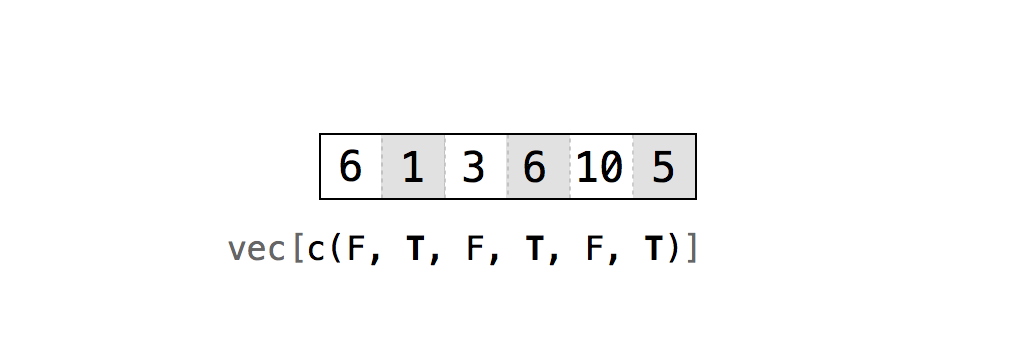
\includegraphics{~/BILD 5 sandbox/Hands_on_programming/hopr_0402.png}
\caption{logical values to subset}
\end{figure}

\begin{Shaded}
\begin{Highlighting}[]
\CommentTok{\#Exercise 6.1 (Deal a Card) Complete the following code to make a function that returns the first row of a data frame:}
\NormalTok{deal }\OtherTok{\textless{}{-}} \ControlFlowTok{function}\NormalTok{(cards) \{}
\NormalTok{  deck[}\DecValTok{1}\NormalTok{, }\FunctionTok{c}\NormalTok{(}\StringTok{"face"}\NormalTok{, }\StringTok{"suit"}\NormalTok{, }\StringTok{"value"}\NormalTok{)]\}}
\FunctionTok{deal}\NormalTok{()}
\end{Highlighting}
\end{Shaded}

\begin{verbatim}
## Error in deal(): object 'deck' not found
\end{verbatim}

\begin{Shaded}
\begin{Highlighting}[]
\CommentTok{\#Exercise 6.2 (Shuffle a Deck) Use the preceding ideas to write a shuffle function. shuffle should take a data frame and return a shuffled copy of the data frame.}

\FunctionTok{shuffle}\NormalTok{(}\AttributeTok{cards =}\NormalTok{ deck)}
\end{Highlighting}
\end{Shaded}

\begin{verbatim}
## Error in shuffle(cards = deck): could not find function "shuffle"
\end{verbatim}

\begin{Shaded}
\begin{Highlighting}[]
\FunctionTok{shuffle}\NormalTok{(deuces.deck)}
\end{Highlighting}
\end{Shaded}

\begin{verbatim}
## Error in shuffle(deuces.deck): could not find function "shuffle"
\end{verbatim}

\#\#\#\#Dollar signs and double brackets

To select a column from a data frame, write the data frame's name and
the column name separated by a \$. Notice that no quotes should go
around the column name.

If the elements in your list do not have names (or you do not wish to
use the names), you can use two brackets, instead of one, to subset the
list. This notation will do the same thing as the \$ notation.

\begin{figure}
\centering
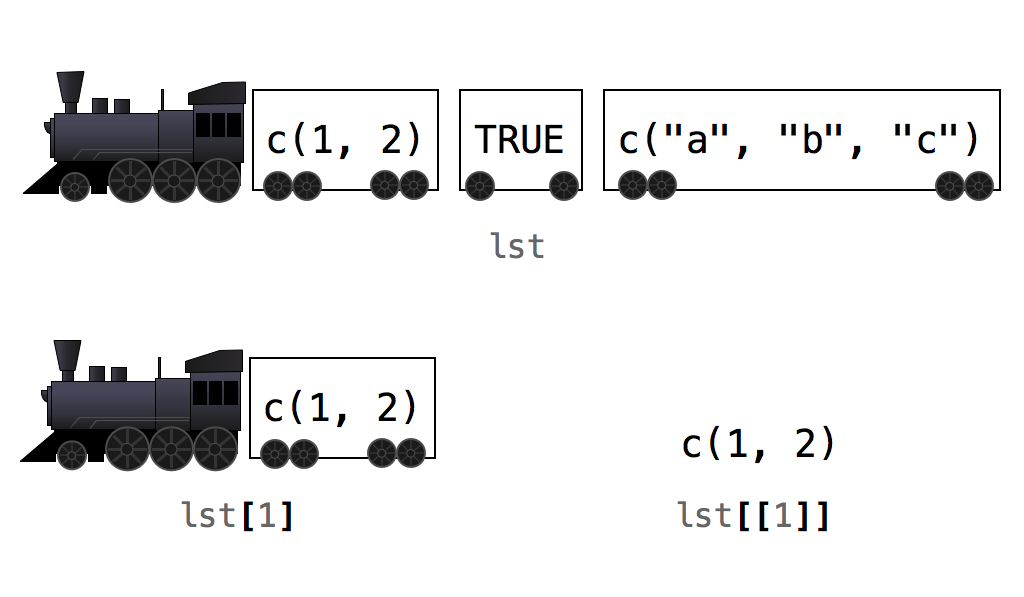
\includegraphics{~/BILD 5 sandbox/Hands_on_programming/hopr_0403.png}
\caption{subsetting - double brackets for lists}
\end{figure}

\begin{Shaded}
\begin{Highlighting}[]
\NormalTok{deck}\SpecialCharTok{$}\NormalTok{value}
\end{Highlighting}
\end{Shaded}

\begin{verbatim}
## Error in eval(expr, envir, enclos): object 'deck' not found
\end{verbatim}

\begin{Shaded}
\begin{Highlighting}[]
\FunctionTok{mean}\NormalTok{(deck}\SpecialCharTok{$}\NormalTok{value)}
\end{Highlighting}
\end{Shaded}

\begin{verbatim}
## Error in mean(deck$value): object 'deck' not found
\end{verbatim}

\begin{Shaded}
\begin{Highlighting}[]
\FunctionTok{median}\NormalTok{(deck}\SpecialCharTok{$}\NormalTok{value)}
\end{Highlighting}
\end{Shaded}

\begin{verbatim}
## Error in median(deck$value): object 'deck' not found
\end{verbatim}

\#\#\#\#Modifying Values

to modify values in a vector ``name of object{[}c(list points you want
to change){]} \textless- c(the new values)

you can even add new variables with
``deck2\(name of new variable <- values" Take it away with "deck2\)name
of new variable \textless- NULL''

What if you need to find data points to change their values, like
changing the value of the aces?

Use \textbf{logical operators}

\begin{longtable}[]{@{}lll@{}}
\toprule
Operator & Syntax & Tests \\
\midrule
\endhead
\textgreater{} & a \textgreater{} b & Is a greater than b? \\
\textgreater= & a \textgreater= b & Is a greater than or equal to b? \\
\textless{} a \textless{} b Is a less than b? & & \\
\textless= a \textless= b Is a less than or equal to b? & & \\
== a == b Is a equal to b? & & \\
!= a != b Is a not equal to b? & & \\
\%in\% a \%in\% c(a, b, c) Is a in the group c(a, b, c)? & & \\
\bottomrule
\end{longtable}

\begin{Shaded}
\begin{Highlighting}[]
\NormalTok{vec }\OtherTok{\textless{}{-}} \FunctionTok{c}\NormalTok{(}\DecValTok{0}\NormalTok{, }\DecValTok{0}\NormalTok{, }\DecValTok{0}\NormalTok{, }\DecValTok{0}\NormalTok{, }\DecValTok{0}\NormalTok{, }\DecValTok{0}\NormalTok{)}
\NormalTok{vec[}\FunctionTok{c}\NormalTok{(}\DecValTok{1}\NormalTok{, }\DecValTok{3}\NormalTok{, }\DecValTok{5}\NormalTok{)] }\OtherTok{\textless{}{-}} \FunctionTok{c}\NormalTok{(}\DecValTok{1}\NormalTok{, }\DecValTok{1}\NormalTok{, }\DecValTok{1}\NormalTok{)}
\NormalTok{vec}
\end{Highlighting}
\end{Shaded}

\begin{verbatim}
## [1] 1 0 1 0 1 0
\end{verbatim}

\begin{Shaded}
\begin{Highlighting}[]
\NormalTok{deck2}\SpecialCharTok{$}\NormalTok{new }\OtherTok{\textless{}{-}} \DecValTok{1}\SpecialCharTok{:}\DecValTok{52}
\end{Highlighting}
\end{Shaded}

\begin{verbatim}
## Error in deck2$new <- 1:52: object 'deck2' not found
\end{verbatim}

\begin{Shaded}
\begin{Highlighting}[]
\NormalTok{deck2}\SpecialCharTok{$}\NormalTok{new }\OtherTok{\textless{}{-}} \ConstantTok{NULL}
\end{Highlighting}
\end{Shaded}

\begin{verbatim}
## Error in deck2$new <- NULL: object 'deck2' not found
\end{verbatim}

\end{document}
